\section{Introduction}

\textbf{Softwerk AB's Coffe Maker}

The coffee maker in Softwerk AB is running with the help of a Raspberry PI, which in turn is controlled via SSH. Right now their system is everything but user friendly and is in need of a upgrade.

\section{Glossary}

\subsection{Raspberry PI}

Small one-card computer with \textit{GPIO} capabilities. Used to give a signal to a \textit{semiconductor relay} to switch the \textit{Moccamaster} on or off.

\subsection{GPIO}

General-Purpose Input/Output - pins that is used with a small electrical current. A GPIO have no special purpose and can be used as it fits the developer best.

In this project some of the pins, probably two of them, is connected to the semiconductor relay.

\subsection{Semiconductor Relay}

The only purpose of the semiconductor relay in this project is to give, or not give, power to the extension cord which is connected to the Moccamaster. The relay provided for this project looks like the picture below.

\vspace{5mm}
\begin{center}
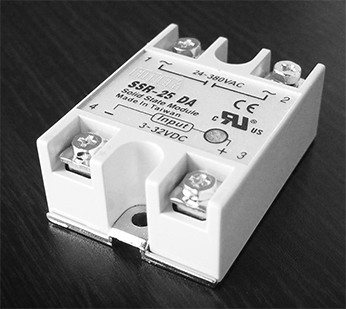
\includegraphics[scale=0.4]{relay}
\end{center}

\subsection{Moccamaster}

The coffee machine used by the company. It's a standard coffee machine with no special functions, and looks like the one below.

\vspace{10mm}

\begin{center}
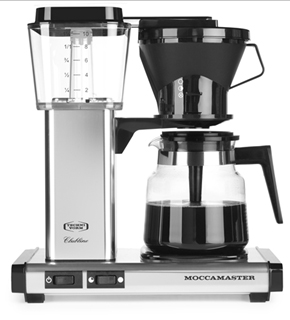
\includegraphics[scale=0.45]{moccamaster}
\end{center}

\subsection{Softwerk AB}

The name of the domain. Softwerk AB has 14 employees, and their CEO is called Eddie Freij.


\section{General Knowledge About the Domain}

\begin{itemize}

\item The process starts the night before, with the last person leaving the building preparing the Moccamaster.
\item The first person arriving at the office triggers the coffe machine remotely.
\item The current system is tedious, and suboptimal, with no user friendly interface.
\item Developers uses SSH over VPN to connect to the Moccamaster.
\item The Raspberry PI uses a semiconductor relay to change the state of the Moccamaster.
\item Currently, there is no way to manually switch the relay on or off, other than plugging the Moccamaster into the wall socket.

\end{itemize}

\section{Customers and Users}

The system is going to be specifically developed for Softwerk AB to satisfy their needs for a more user friendly solution with statistics and an administrator section. Thus, the only users will be the employees of Softwerk AB.

\section{The Environment}

\begin{itemize}

\item The actors all have a cellphone which they can control the Moccamaster with.
\item The actors may use their PCs to switch the relay.
\item The semiconductor relay has two states - on/off.

\end{itemize}

\section{Tasks and Procedures Currently Performed}

Currently, there the functions of the solution are limited to a few. The tasks performed are listed below.

\subsection{Switch the State}

\begin{enumerate}
\item Connect via VPN.
\item Login via SSH.
\item Write a command to switch the state.
\item Log out.
\end{enumerate}

\subsection{Manual Override}
\begin{enumerate}
\item Disconnect the Moccamaster from the extension cord.
\item Plug it into the wall socket.
\end{enumerate}

\subsection{Manual Override - Reset}
\begin{enumerate}
\item Disconnect the Moccamaster from the wall socket.
\item Plug it into the extension cord.
\end{enumerate}

\section{Competing Solutions}

Competing software are so called \textit{Smart Coffe Machines}. They are basically coffee machines with WIFI capabilities, allowing the possibility to connect to the coffee machine remotely.

The most basic machines allows the ability switch the state on or off, and allows scheduling when to make the coffee. The more sophisticated ones opens up the machine for social media, such as updating on Facebook and Twitter when the coffee machine is done and so forth.

One major difference between the solution in this domain and the solution in other domain is the fact that this one is without doubt the cheapest solution money wise. A basic coffee machine with WIFI costs almost three times as much as this domain's solution cost to build.
